%!TEX root = ../thesis.tex
\chapter{Detalles de implementación} % (fold)
\label{cha:detalles_de_implementacion}
	En este capítulo se explica cómo fueron implementados \textit{Beampress} y \textit{Beampressk} tomando en cuenta los requerimientos vistos en la sección \ref{sec:requerimientos_basicos_del_sistema_propuesto}, y siguiendo las concepciones definidas en el capítulo anterior. Se describe cómo se confecciona una presentación en HTML y cómo el \textit{plugin} de jQuery \textit{beampress.js} la interpreta. Se muestra cómo se implementan las funciones de transición, y las características de dicho \textit{plugin}.

	Se analiza, de \textit{Beampressk}, la implementación del servidor web en Flask, cómo se definen la vista de control, de presentación, el modo en que se utilizó \textit{WebSocket} como tecnología para un canal de comunicación bidireccional entre estas, así como las funcionalidades de \textit{Beampressk} como API REST.

	Al definir la presentación en ámbito web, se aprovechan las bondades de HTML5 y CSS3 para conformar las diapositivas separando contenido de forma. A continuación se explica cómo estructurar una presentación y se detallan las características del \textit{plugin} de jQuery \textit{beampress.js}. 

	\section{Beampress} % (fold)
	\label{sec:beampress_imp}
	

		Como se describió en la sección \ref{sec:beampress} se utilizó un patrón ligero como diseño para la implementación de \textit{beampress.js}. 

		En esta sección se explica cómo crear contenidos, \textit{slide items}, \textit{overlays} y \textit{frames}.

		Para crear una presentación siguiendo las definiciones del capítulo anterior, se hace uso de las etiquetas y atributos de HTML.


		\subsection{Contenidos} % (fold)
		\label{sub:contenidos}
			Los contenidos de la presentación son cualquier elemento de HTML que se especifique, por ejemplo un \textit{párrafo} (\texttt{<p>}), una \textit{imagen} (\texttt{<img>}), un \textit{video} (\texttt{<video>}), un \textit{audio} (\texttt{<audio>}) o un \textit{canvas} (\texttt{<canvas>}). En la fig. \ref{fig:frames_html_content} se muestran ejemplos de contenidos en HTML.

				\begin{figure}[htb]%

					\begin{lstlisting}						
<!-- Texto -->
<p>Un texto</p>

<!-- Imagen -->
<img src="imagen.jpg" alt="imagen">

<!-- Video -->
<video src="video.mp4"></video>

<!-- Audio -->
<audio src="sound.mp3"></audio>		 							 					
 					 			

					\end{lstlisting}
					\caption{Contenidos de un \textit{frame} en HTML}
					\label{fig:frames_html_content}
				\end{figure}	  
		
		% subsection contenidos (end)


		\subsection{Overlays y Slide Items} % (fold)
		\label{sub:slide_items}
			Según la definición \ref{def:slide_item}, un \textit{slide item} es un contenido con un conjunto de \textit{overlays}. Para emplear la sintaxis de \textit{overlays} vista en el ejemplo \ref{ex:overlay_set} se hace uso de los atributos \texttt{data} de HTML5, para lo cual se definió el atributo \texttt{data-onslide}. Un \textit{slide item} es un contenido de HTML con el atributo \texttt{data-onslide}, que tiene como valor el conjunto de \textit{overlays} usando la sintaxis básica del ejemplo \ref{ex:overlay_set}, o la sintaxis extendida vista en la sección \ref{subsec:sintaxis_extendida}. Como ejemplo, en la fig. \ref{fig:slide_items_html} se definen varios \textit{slide items} usando la sintaxis básica.


				\begin{figure}[htb]%
					\begin{lstlisting}%

<img data-onslide="1-" src="test.jpg" alt="test">
<ul>
    <li data-onslide="3-">Desde el slide 3 hasta el final</li>
    <li data-onslide="4;6">En el slide 4 y 6</li>
    <li data-onslide="5;8">En el slide 5 y 8</li>
    <li data-onslide="3-5;7-8">Del 3 al 5 y del 7 al 8</li>
</ul> 

	
					\end{lstlisting}
					\caption{Forma de definir \textit{slide items} con \textit{overlays} en HTML5}
					\label{fig:slide_items_html}
				\end{figure}
			Un \textit{slide item} está mostrado en todos los \textit{slides} si no tiene \textit{overlays}, o sea, si un elemento HTML no tiene el atributo \texttt{data-onslide} se mostrará en todas las transiciones del \textit{frame} al que pertenece. En caso de tenerlo, se ocultará en todos los \textit{slides} a no ser que sus \textit{overlays} determinen otra conducta.


			Para determinar los \textit{slides} de un \textit{frame}, \textit{beampress.js} primero analiza todos elementos HTML hijos de dicho \textit{frame} y en dependencia de cada conjunto de \textit{overlays}, obtiene el menor y el mayor \textit{slide}, que son el primero y el último respectivamente.

			Para analizar cada \textit{overlay} con la sintaxis básica, se utiliza la siguiente expresión regular: \texttt{/([1\textendash 9]\textbackslash d*)?(\textendash )?([1\textendash 9]\textbackslash d*)?/} para agrupar los límites inferior y superior. Nótese que estos pueden no estar, al igual que puede ser sólo un número sin \texttt{\textendash}. 

			Un \textit{overlay} es un objeto JSON con el mismo formato de la fig. \ref{fig:json_format} y teniendo en cuenta la definición \ref{def:new_overlay}, determina una función de transición siguiente y una función de transición anterior para uno o varios \textit{slides}. El \textit{plugin} \textit{beampress.js} transforma la sintaxis básica en la sintaxis extendida de la sección \ref{subsec:sintaxis_extendida}. 

			Por ejemplo, si se tiene el siguiente conjunto de \textit{overlays}: $$-2; 4$$ \textit{beampress.js} lo convierte en los \textit{overlays} de la fig. \ref{fig:overlay_set_beampress}. Las funciones elementales se implementaron en \textit{beampress.js} de forma tal que modifican el atributo \texttt{opacity} del elemento en cuestión.

				\begin{figure}[htb]%
					\begin{lstlisting}%

// Slide 1
{"1":{"siguiente":{"func": "mostrar", "args": {}},
      "anterior": {"func": "ocultar", "args": {}}}} 
// Slide 2
{"2":{"siguiente":{"func": "identidad", "args": {}},
      "anterior": {"func": "identidad", "args": {}}}}  
// Slide 3
{"3":{"siguiente":{"func": "ocultar", "args": {}},
      "anterior": {"func": "mostrar", "args": {}}}}  
// Slide 4
{"4":{"siguiente":{"func": "mostrar", "args": {}},
      "anterior": {"func": "ocultar", "args": {}}}}                                       				
	
					\end{lstlisting}
					\caption{Representación en beampress.js del conjunto de \textit{slides} \texttt{-2; 4}}
					\label{fig:overlay_set_beampress}
				\end{figure}			
					
		
			
			Debe aclararse que al definir los \textit{overlays} usando la sintaxis extendida, \textit{beampress.js} parsea explícitamente el \textit{overlay}, para convertirlo en objeto JSON. Como ejemplo, en la fig. \ref{fig:extended_syntax_html} se muestran \textit{slide items} que tienen definidos sus \textit{overlays} con la sintaxis extendida.

			\begin{figure}[htb]%
				\begin{lstlisting}%

<!-- Slide 4 -->
<span data-onslide='{
    "4": {
        "next": {
            "func": "slowShowItem",
            "args": {}
        },
        "prev": {
            "func": "slowHideItem",
            "args": {}
        }
    }}'>
	Leve transición en el \textit{slide} 4
</span>

<!-- Slide 2 -->
<span data-onslide='{
    "2": {
        "next": {
            "func": "slowShowItem",
            "args": {}
        },
        "prev": {
            "func": "slowHideItem",
            "args": {}
        }
    }}'>
	Leve transición en el \textit{slide} 2
</span>

			
				\end{lstlisting}
				\caption{Uso de la sintaxis extendida en \textit{slide items}.} 
				\label{fig:extended_syntax_html}
			\end{figure}

			En la fig. \ref{fig:basic_and_extended_syntax_html} se exhibe un \textit{slide item} que tiene especificado sus \textit{overlays} usando la sintaxis extendida y la sintaxis básica.


			\begin{figure}[htb]%
				\begin{lstlisting}%

<span data-onslide='-2;{
    "4": {
        "next": {
            "func": "slowShowItem",
            "args": {}
        },
        "prev": {
            "func": "slowHideItem",
            "args": {}
        }
    }}'>
	Hasta el \textit{slide} 2 y luego en el \textit{slide} 4
</span>

			
				\end{lstlisting}
				\caption{Uso de ambas extendida en un \textit{slide item}.} 
				\label{fig:basic_and_extended_syntax_html}
			\end{figure}			


			Las funciones de transición \texttt{slowShowItem} y \texttt{slowHideItem} utilizadas en la fig. \ref{fig:extended_syntax_html} no son las elementales, pero están definidas en \textit{beampress.js}. Con el fin de cumplir los requerimientos de la sección \ref{sec:requerimientos_basicos_del_sistema_propuesto} se implementaron otras funciones además de las elementales. Como invariante estas funciones reciben en sus argumentos el selector DOM del elemento que modifican. A continuación se describe el efecto que produce cada una en el elemento a modificar:

			\begin{itemize}
				\item \texttt{addStyle(\$el, args)}: Agrega los estilos CSS que recibe como argumentos
				\item \texttt{removeStyle(\$el, args)}: Elimina todos los estilos CSS definidos
				\item \texttt{slowShowItem(\$el, args)}: Realiza un \texttt{animate} de jQuery incrementando la opacidad hasta el 100 \% del elemento con el tiempo especificado en los argumentos
				\item \texttt{slowHideItem(\$el, args)}: Realiza un \texttt{animate} de jQuery disminuyendo la opacidad del elemento con el tiempo especificado en los argumentos
				\item \texttt{playAudio(\$el, args)}: Reproduce el audio en el tiempo y con el volumen especificados en los argumentos
				\item \texttt{stopAudio(\$el, args)}: Detiene el audio
				\item \texttt{playVideo(\$el, args)}: Reproduce el video en el tiempo y con el volumen especificados en los argumentos
				\item \texttt{stopVideo(\$el, args)}: Detiene el video
				\item \texttt{slowShowFrame(\$el, args)}: Similar a \texttt{slowShowItem} pero además establece el valor de \texttt{display} en \texttt{Blovk}
				\item \texttt{slowHideFrame(\$el, args)}: Similar a \texttt{slowHideItem} pero además establece el valor \texttt{display} en \texttt{none}				
			\end{itemize}
			En el capítulo \ref{cha:extensibilidad} se explica el modo en que se pueden agregar otras funciones que se definan, así como el formato que deben tener.

			En \textit{beampress.js} un \texttt{slide item} es un objeto de JavaScript ~\cite{book:1047044} de tipo \texttt{SlideItem} con las siguientes propiedades:

			\begin{itemize}
			\label{it:slide_item}
			 	\item \texttt{\$el}: selector jQuery del elemento HTML que representa
			 	\item \texttt{overlays}: lista de todos los objetos JSON que definen sus \textit{overlays}
			 	\item función \texttt{next}: recibe el número del \textit{slide} actual como argumento del \textit{frame} mostrado. Ejecuta la función \textit{siguiente}, cuyo nombre está determinado por el \textit{overlay} que tiene como llave el \textit{slide} del argumento 
			 	\item función \texttt{prev}: recibe el número del \textit{slide} actual como argumento del \textit{frame} mostrado y ejecuta la función \textit{anterior}			 	
			 \end{itemize} 
				
		% subsection \textit{slide}_items (end)	

		\subsection{Frames} % (fold)
		 \label{sub:frames}
		 
		  
			Un \textit{frame} es un contenedor con la clase \texttt{frame}, y el orden en que se muestra cada uno es el mismo con el que se define. En la fig. \ref{fig:frames_html} se muestran varios \textit{frames}.


				\begin{figure}[htb]%
					\begin{lstlisting}%

<section class="frame">Primer Frame</section>
<section class="frame">Segundo Frame</section>
<!-- ... -->
<section class="frame">Enésimo Frame</section>
					\end{lstlisting}
					\caption{Forma de definir \textit{frames} en HTML}
					\label{fig:frames_html}
				\end{figure}

			Los \textit{slide items} de cada contenedor \textit{frame} se definen dentro del mismo, o sea, son sus hijos. Cada \textit{frame} es un objeto de JavaScript de tipo \texttt{Frame} que hereda de \texttt{SlideItem}.


			 % para adquirir las propiedades vistas en el listado \ref{it:slide_item}. 
			Con el propósito de organizar la presentación \textit{beampress.js} analiza cada \textit{frame} empleando el selector \texttt{\$(".frame")} y por cada uno crea un objeto \texttt{Frame}. Para obtener los \textit{slide items} con conjunto de \textit{overlays} en un \textit{frame}, o sea, todos los elementos HTML hijos de un contenedor \textit{frame} con el atributo \texttt{data-onslide}, se utiliza el selector \texttt{\$("[data-onslide]")} y por cada uno se crea un objeto \texttt{SlideItem}. Las instancias de \texttt{Frame} son almacenadas en una lista y en todo momento se sabe qué \textit{frame} está mostrado y en qué \textit{slide} se encuentra con los índices \texttt{currentFrame} y \texttt{currentSlide} respectivamente.

			Un objeto \texttt{Frame} tiene una lista de objetos \texttt{SlideItem}. Sus funciones de transición o transiciones de entrada y salida por defecto se hacen alterando su atributo \texttt{display}, que en caso de estar mostrado es \texttt{block} y en caso contrario es \texttt{none}. Un \textit{frame} hace su transición de salida cuando se visualizan todos sus \textit{slides} y el siguiente (en caso de existir) realiza su transición de entrada. En la fig. \ref{fig:frame_html_slides} se muestra un \textit{frame} con varios \textit{slide items}.

			\begin{figure}[htb]%
				\begin{lstlisting}%

<section class="frame">
	<h1>Frame</h1>
	<span data-onslide="1-">Texto1</span>
	<span data-onslide="2-">Texto2</span>
	<span data-onslide="3-">Texto3</span>
</section>
				\end{lstlisting}
				\caption{Un \textit{frame} en HTML con varios \textit{slide items}}
				\label{fig:frame_html_slides}
			\end{figure}

			El \textit{slide item} \texttt{<h1>Frame</h1>} de la fig. \ref{fig:frame_html_slides} siempre estará visible en todos los \textit{slides} del \textit{frame} porque no tiene definido un conjunto de \textit{overlays}. En otras palabras: no presenta el atributo \texttt{data-onslide} y como consecuencia, no se crea ningún objeto \texttt{SlideItem} porque no está en los resultados del selector \texttt{\$("[data-onslide]")}.


			En la sección \ref{subsec:sintaxis_extendida} se argumentó que un \textit{frame} podía tener funciones de transición, en este caso, transición de entrada y salida. Usando la sintaxis extendida y los atributos \texttt{data-onshow} y \texttt{data-onhide} se puede efectuar dicha funcionalidad. En la fig. \ref{fig:frames_transitions} se ejemplifican dos \textit{frames} con transiciones de entrada y de salida.


		\begin{figure}[htb]%
			\begin{lstlisting}%

<section data-onhide='{"func": "slowHideFrame", "args": {}}' class="frame"></section>
<section data-onshow='{"func": "slowShowFrame", "args": {}}' class="frame"></section>
			\end{lstlisting}
		\caption{Transiciones entre \textit{frames}}
		\label{fig:frames_transitions}
		\end{figure}	

		El \textit{plugin} \textit{beampress.js} realiza las transiciones de los \textit{frames} de forma similar a la manera en que las realiza con los \textit{slide items}, pero sin depender de un \textit{slide}.
		% subsection \textit{frames} (end)

		\subsection{Transiciones} % (fold)
		\label{sub:transiciones}
			Para realizar las transiciones o cambio de \textit{slides}, se implementaron las funciones \texttt{next()} y \texttt{prev()} que efectúan las transiciones siguiente y anterior respectivamente. Estas funciones están registradas a distintos eventos, de forma tal que se ejecutan en dependencia de la interacción del usuario con el navegador, o de la interacción de algún otro dispositivo utilizando \textit{WebSocket}. Esto último se explicará con más detalle en la sección \ref{sec:beampressk_imp}.
		% subsection transiciones (end)

		\subsection{Presentación} % (fold)
		\label{sub:presentacion}

			Todos los \textit{frames} de la presentación van contenidos en el objeto DOM que instancia al \textit{plugin} \textit{beampress.js}. En la fig. \ref{fig:main_container} se define un \texttt{<div>} con clase \texttt{main-container} que contiene los \textit{frames} de una presentación. Usando este ejemplo, se instancia al \textit{plugin} de la siguiente manera:\\ \texttt{\$(".main-container").beampress();} como se muestra en la fig. \ref{fig:ex5}.
		
			\begin{figure}[htb]%
				\begin{lstlisting}%

<div class="main-container">
	<!-- Los Frames van aquí -->
</div>
				\end{lstlisting}
			\caption{Contenedor principal}
			\label{fig:main_container}
			\end{figure}				


			Como \textit{beampress.js} está basado en jQuery, para usarlo es necesario incluir alguna biblioteca de jQuery. Un ejemplo completo de su uso puede verse en la Fig. \ref{fig:ex5}

			\begin{figure}[htb]%
				\begin{lstlisting}%

<!DOCTYPE html>
<html>
	<head>
    	<title>Ejemplo</title>
	</head>
	<body>
		<div id="main-container">
			<section class="frame">
				<!-- Contenido del \textit{frame} -->
			</section>
			<section class="frame">
				<!-- Contenido del \textit{frame} -->
			</section>						
		</div>
	   <script src="js/jquery-1.10.2.min.js"></script>
	   <script src="js/beampress.js"></script>
	   <script>
	       $(document).ready(function(){     
	           $(".main-container").beampress();
	        });
	   </script>		
	</body>
</html>			
				\end{lstlisting}
			\caption{
				Ejemplo de presentación usando \textit{beampress.js}. 
				\label{fig:ex5} }
			\end{figure}	

			El estilo de la presentación queda sujeto al usuario, por lo que se requieren previos conocimientos de HTML, CSS y JavaScript. Como extensión a la propuesta de este trabajo se implementó el estilo Warsaw de \textit{Beamer} con el CSS \texttt{warsaw.css} que se mencionará también en la siguiente sección.
		% subsection presentación (end)
	% section beampress (end)

	\section{Beampressk} % (fold)
	\label{sec:beampressk_imp}
		Se implementó una aplicación de \textit{Flask} para manejar todos los pedidos que el servidor web recibe usando el protocolo \textit{Web Server Gateway Interface} (WSGI). La instancia de la aplicación es un objeto de clase \textit{Flask}.

		La aplicación asocia URLs con funciones de Python que tenga definidas. Dicha asociación se llama \textit{ruta} y en esta sección se asume \texttt{beampress.com} como URL base.
		
		\subsection{Estructura de la aplicación} % (fold)
		\label{sub:estructura_de_la_aplicacion}
			Todas las vistas que se definieron en la sección \ref{sec:definiciones_de_beampressk} se conforman usando el sistema de \textit{templates} \textit{Jinja2}, en la fig. \ref{sub:estructura_de_la_aplicacion} se muestra la ubicación de cada \textit{template}.
			Para interpretar las presentaciones, o sea, interpretar los \textit{frames}, \textit{slides}, \textit{slide items}, \textit{overlays} y las funciones de transición se usa el \textit{plugin} \textit{beampress.js} cuyas características se argumentaron en la sección anterior. El uso de \textit{SocketIO} ~\cite{socketio} se realiza con la biblioteca \textit{socket.io.min.js}. Para eliminar los 300ms de espera en los navegadores móviles desde el momento en que se toca un botón para disparar el evento \texttt{click}, se usa \texttt{fastclick.js} ~\cite{fastclick}. La razón de este retraso es que el navegador espera ese tiempo para determinar si se hace un doble click ~\cite{fior}.
			\begin{figure}[htb]%
				\dirtree{%
				.1 beampressk.
				.2 static \ldots{} \begin{minipage}[t]{8cm}
									\textit{Todos los recursos se localizan aquí}{.}
								\end{minipage}.
				.3 css.
				.4 warsaw{.}css \ldots{} \begin{minipage}[t]{8cm}
									\textit{CSS para el estilo de Warsaw}{.}
								\end{minipage}.	
				.3 js.
				.4 beampress{.}js \ldots{} \begin{minipage}[t]{8cm}
									\textit{Plugin de Beampress}{.}
								\end{minipage}.
				.4 socket{.}io{.}min{.}js \ldots{} \begin{minipage}[t]{8cm}
									\textit{Biblioteca para SocketIO}{.}
								\end{minipage}.
				.4 fastclick{.}js \ldots{} \begin{minipage}[t]{8cm}
									\textit{Biblioteca Fastclick}{.}
								\end{minipage}.
				.2 templates.
				.3 nombre\_de\_pres \ldots{} \begin{minipage}[t]{8cm}
									\textit{Ejemplo de una presentación}{.}
								\end{minipage}.
				.4 index{.}html.
				.3 warsaw\_base{.}html \ldots{} \begin{minipage}[t]{8cm}
									\textit{Template base para todas las presentaciones con estilo Warsaw}{.}
								\end{minipage}.
				.3 index{.}html \ldots{} \begin{minipage}[t]{8cm}
									\textit{Template de la vista de control}{.}
								\end{minipage}.	
				.2 app{.}py \ldots{} \begin{minipage}[t]{8cm}
									\textit{La aplicación de Flask}{.}
								\end{minipage}.				
				}

			\caption{Estructura de Beampressk}
			\label{fig:beampressk_structure}
			\end{figure}		
		% subsection estructura_de_la_aplicación (end)

		\subsection{Presentaciones} % (fold)
		\label{sub:presentaciones}

			Por convenio, un \textit{template} de presentación debe llamarse \texttt{index.html} y encontrarse en una carpeta con el nombre de la presentación, que a su vez tiene que estar contenida en el directorio \texttt{templates} como se muestra en la fig. \ref{fig:beampressk_structure}. Para mostrar cada presentación se usa la siguiente URL: \\
			\texttt{beampressk.com/presentation/nombre\textendash de\textendash presentacion} y esta es analizada por la aplicación de \textit{Flask} (\texttt{app.py}) con la función \texttt{show} de la fig. \ref{fig:presentation_routes}.

			La presentación será visualizada en varios clientes si estos acceden a la misma URL que la representa. 

			\begin{figure}[htb]%
				\begin{lstlisting}[language=Python]%

# Presentaciones
@app.route('/presentation/<name>')
def show(name):
    return render_template('%s/index.html' % name)
				\end{lstlisting}
			\caption{Rutas dinámicas para las presentaciones}
			\label{fig:presentation_routes}
			\end{figure}

		% subsection presentaciones (end)

		\subsection{Vista de control} % (fold)
		\label{sub:vista_de_control}
			El \textit{template} de la vista de control se encuentra en \texttt{templates/index.html} como se muestra en la fig. \ref{fig:beampressk_structure} y su URL es \texttt{beampress.com}. La función \texttt{index} de la fig. \ref{fig:control_view_code} es llamada, luego de acceder a la URL raíz.

			\begin{figure}[htb]%
				\begin{lstlisting}[language=Python]%

# Vista de control
@app.route('/')
def index():
    return render_template('index.html')
				\end{lstlisting}
			\caption{Ruta para la vista de control}
			\label{fig:control_view_code}
			\end{figure}

			En la fig. \ref{fig:control} se muestra la vista de control visualizada en un dispositivo móvil.

			\begin{figure}[tb]
				\centering
				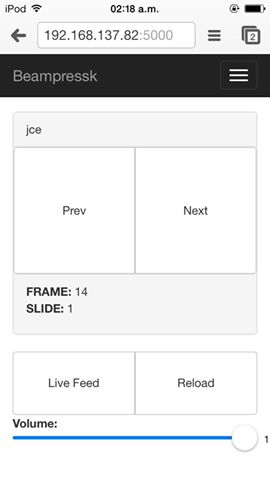
\includegraphics[width=6cm]{img/control}
				\caption{Ejemplo de la vista de control visualizada en un dispositivo móvil}
				\label{fig:control}
			\end{figure}						
		% subsection vista_de_control (end)

		\subsection{WebSocket} % (fold)
		\label{sub:websocket}

		En la sección \ref{sec:definiciones_de_beampressk} se definió que la comunicación entre la vista de control y la vista de presentación tenía que ser instantánea. Como se vio en la sección \ref{sec:beampressk} se utilizó \textit{WebSocket} para establecer un canal de comunicación bidireccional entre estas vistas. Para ello se incluyó la extensión de Flask \textit{Flask-SocketIO} ~\cite{flasksocket} en la aplicación de Beampressk que establece una conexión con los clientes que tengan la biblioteca \textit{Socket.IO}.

			\subsubsection{Mensajes de comunicación} % (fold)
			\label{ssub:mensajes_de_comunicacion}
				Para establecer la comunicación entre la vista de control y la vista de presentación se usan los mensajes de \textit{SocketIO}. Estos mensajes son registrados con \textit{Flask-SocketIO} de forma similar a la manera en que registra las \textit{rutas} con funciones de Python. 

				De esta manera la aplicación de \textit{Flask} funciona como intermediaria entre la vista de control y la vista de presentación. Los mensajes definidos en la tabla \ref{tab:messages} se muestran en la fig. \ref{fig:control_view_msgs} y \ref{fig:presentation_view_msgs} para la parte cliente y en la fig. \ref{fig:server_msgs} para la parte servidor.


			\begin{figure}[htb]%
				\begin{lstlisting}[language=JavaScript]%

// Evento ante 'respuesta actualiza'
socket.on('response', function(msg) {
    // Actualizar información acerca 
    // de la presentación
}); 

// Mensaje 'siguiente'
socket.emit('next');

// Mensaje 'anterior'
socket.emit('prev');

// Mensaje 'volumen'
socket.emit('volume', {data: <valor-volumen>});

// Mensaje 'live feed'
socket.emit('live_feed');

// Mensaje 'message'
socket.emit('hide_msg');
  
				\end{lstlisting}
			\caption{Mensajes de comunicación en la vista de control}
			\label{fig:control_view_msgs}
			\end{figure}

			\begin{figure}[htb]%
				\begin{lstlisting}[language=JavaScript]%

// Mensaje 'siguiente'
socket.on('next_response', function() {
	// Transición siguiente
	next();
	// Mensaje 'respuesta actualiza'
	socket.emit('update_info', {data: <información>});
});


// Mensaje 'anterior'
socket.on('prev_response', function() {
	// Transición anterior
	prev();
	// Mensaje 'respuesta actualiza'
	socket.emit('update_info', {data: <información>});
});


//Mensaje 'volumen'
socket.on('volume_response', function(msg) {
	// Actualizar volumen
});

//Mensaje 'live feed'
socket.on('live_feed_response', function() {
    // Mostrar u ocultar el live feed
});

//Mensaje 'message'
socket.on('msg', function(msg){
	// Mostrar mensaje
});

//Mensaje 'message'
socket.on('hide_msg_response', function (){
	// Ocultar mensaje
}); 
  
				\end{lstlisting}
			\caption{Mensajes de comunicación en la vista de presentación}
			\label{fig:presentation_view_msgs}
			\end{figure}

			\begin{figure}[htb]%
				\begin{lstlisting}[language=Python]%

# Mensaje respuesta actualiza
@socketio.on('update_info', namespace='/beampressk')
def beampressk_update_info(message):
    data = message.get('data', {})
    emit('response', {'data': data}, broadcast=True)

# Mensaje siguiente
@socketio.on('next', namespace='/beampressk')
def beampressk_next():
    emit('next_response', broadcast=True)

# Mensaje anterior
@socketio.on('prev', namespace='/beampressk')
def beampressk_prev():
    emit('prev_response', broadcast=True)

# Mensaje volumen
@socketio.on('volume', namespace='/beampressk')
def beampressk_volume(message):
    emit('volume_response', {'data': message.get('data', {})}, broadcast=True)

# Mensaje live feed
@socketio.on('live_feed', namespace='/beampressk')
def beampressk_live_feed():
    emit('live_feed_response', broadcast=True)

# Mensaje message
@socketio.on('hide_msg', namespace='/beampressk')
def beampressk_hide_msg():
    emit('hide_msg_response', broadcast=True)
  
				\end{lstlisting}
			\caption{Mensajes de comunicación en el servidor}
			\label{fig:server_msgs}
			\end{figure}							

			% subsubsection mensajes (end)		

		\subsection{Live Feed} % (fold)
		\label{sub:live_feed}

			La captura multimedia HTML (audio y video) se realiza con la API \texttt{getUserMedia()} que funciona en combinación con las etiquetas de HTML5 \texttt{<audio>} y \texttt{<video>}. El primer parámetro de \texttt{getUserMedia()} especifica el tipo de medio al que se quiere acceder. Por ejemplo, si se quiere solicitar la cámara web, el primer parámetro debe ser \texttt{video}. Para usar tanto el micrófono como la cámara, se utiliza \texttt{video, audio}.

			Como se observó en las fig. \ref{fig:control_view_msgs}, \ref{fig:presentation_view_msgs} y \ref{fig:server_msgs} se puede activar o desactivar un \textit{live feed} mediante los mensajes de \textit{WebSocket}. A continuación se explica el uso de esta funcionalidad mediante otro servicio web, así como la incorporación de otros contenidos en la presentación utilizando las rutas de la aplicación en \textit{Flask}.
		
		% subsection live_feed (end)
		
		% subsection websockets (end)

		\subsection{API REST} % (fold)
		\label{sub:api_rest_imp}
			En la sección \ref{sub:api_rest} se explicaron las características de un servicio REST, cuya concepción está centrada en la noción de recursos. Para almacenar información referente a la presentación como el \textit{frame} y el \textit{slide} actual, así como el volumen de los elementos multimedia de la misma, se utiliza una estructura de memoria. Esta estrategia es factible ya que \textit{Beampressk} no es un servidor web en producción, con una gran cantidad de accesos.

			Para efectuar un método POST y emitir un mensaje de \textit{WebSocket} se usa la función de la fig. \ref{fig:post_method}. De esta manera se puede activar el \textit{live feed} o mostrar mensajes de texto que se envíen en el pedido. En la fig. \ref{fig:curl_post} se efectúa un pedido POST usando \texttt{curl}.

			\begin{figure}[htb]%
				\begin{lstlisting}[language=Python]%

# pedidos RESTfuls

# POST
@app.route('/action', methods=['POST'])
def beampressk_emit_task():
    action = request.json['action']
    if action == 'live_feed':
        socketio.emit('live_feed_response', namespace='/beampressk')
    elif action == 'msg':
        data = request.json['data']
        socketio.emit('msg', {'data': data}, namespace='/beampressk')
    return jsonify({'action': action}), 200  
  
				\end{lstlisting}
			\caption{Método POST}
			\label{fig:post_method}
			\end{figure}			

			\begin{figure}[htb]%
				\begin{lstlisting}[language=Python]%

$ curl -i -H "Content-Type: application/json" -X POST -d '{"action":"msg", "data":"Este es un mensaje de texto"}' http://beampressk.com:5000/action
  
				\end{lstlisting}
			\caption{Método POST usando curl}
			\label{fig:curl_post}
			\end{figure}
			
			
		% subsection api_rest (end)	
	% section beampressk (end)

	En este capítulo fueron analizados, de \textit{Beampress} sus características, sus funcionalidades y el modo en que es capaz de interpretar las presentaciones. Por su parte, de \textit{Beampressk} se explicó su implementación como servidor web en Flask, se definieron las vistas de control y de presentación destacando la instantaneidad lograda entre ambas al configurar un canal bidireccional de comunicación utilizando \textit{WebSocket}.

	Seguidamente se muestra cómo puede definirse cualquier función de animación en JavaScript, vinculándose a \textit{Beampress}, así como una forma genérica de agregar funcionalidades para la API REST que provee \textit{Beampressk}.
		
% chapter detalles_de_implementacion (end)